\subsection{Question 1}

\subsubsection{Point 1}

\begin{equation}
	\begin{aligned}
		f(x) &= \frac{1}{C - x} + x\\
		f(2) &= 1\\
		1 &= \frac{1}{C - 2} + 2\\
		C &= 1
	\end{aligned}
\end{equation}

// TO DO : calcul de stabilité

\subsubsection{Point 2}

\begin{equation}
	\begin{aligned}
		f_2 &= 1\\
		f_{i+1} &= h(1 + (x_i - f_i)^2)+f_i\\
	\end{aligned}
\end{equation}

// TO DO : calcul de h

\subsubsection{Point 3}

\code{littleclasses}{ForwardEuler.java}

Pour adapter le code à une autre fonction, il faut modifier les variables au début ainsi que la méthode \texttt{F}. Il est également possible de mettre la fonction exacte dans la méthode \texttt{exactFunction} et de mettre le booléen \texttt{compareWithExactFunction} à \texttt{true}. Dans ce cas, un deuxième fichier est créé contenant les valeurs calculées avec la fonction exacte. On peut alors créer un graphe pour les comparer avec gnuplot par exemple via la commande suivante :
\begin{lstlisting}
plot 'forward_euler.txt' with lines, 'exact_function.txt' with lines
\end{lstlisting}

\begin{figure}[H]
	\caption{\label{12_forward_1} Forward Euler avec $h=0.25$}
	\centering
	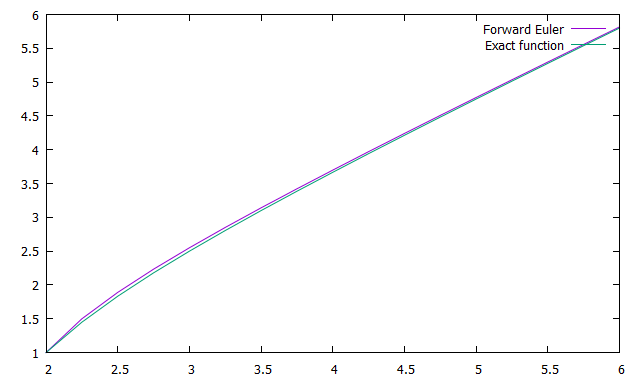
\includegraphics[scale = 0.6]{12_forward_1.png}
\end{figure}


\subsection{Question 2}

// TO DO

\subsection{Question 3}

// TO DO

\subsection{Question 4}

// TO DO